% This work is licensed under the Creative Commons
% Attribution-NonCommercial 3.0 Unported License. To view a copy of this
% license, visit http://creativecommons.org/licenses/by-nc/3.0/.

\section{Auswertung}

\subsection{Messung des Kontrasts}

Zur Auswertung der Meßdaten, die sich bei Kontrastmessung ergeben haben,
benutzen wir eine nichtlineare Ausgleichsrechnung\footnote{%
  Die numerische Berechnung wird von der Funktion
  \texttt{scipy.optimize.curve\_fit} aus der Python-Bibliothek
  \texttt{scipy} in der Version 0.10.1 durchgeführt}.
%
Die zu messenden Intensitäten wurden über entsprechend proportionale
Spannungen bestimmt.  Wir nehmen einen Zusammenhang $U = f(\phi)$
zwischen $\phi$ und den gemessenen Spannungen an, der durch die Funktion
$f\colon [0,\pi] \to \R$ mit
%
\begin{equation}
  \label{eq:contrast_reg}
  f(\phi) = A \pm A\sin(2 \phi + B) + C
\end{equation}
%
gegeben ist.  Im Fall der maximalen Intensität wird das positive
Vorzeichen gewählt, im anderen Fall das negative.  Diese Funktion ergibt
sich wegen \eqref{eq:intens_max} und \eqref{eq:intens_min} aus dem
Theorieteil.  Die Ergebnisse der Ausgleichsrechnung sind in
\cref{tab:intensity} und \cref{fig:intensity} dargestellt.

In \cref{fig:contrast} ist der Kontrast in Abhängigkeit des
Polarisationswinkels dargestellt.  In den Plot ist zum Vergleich die
Funktion $\sin(2x)$ eingezeichnet, da diese gemäß den Formeln
\eqref{eq:kontrast}, \eqref{eq:intens_max} und \eqref{eq:intens_min} die
Abhängigkeit zwischen Kontrast und Polarisationswinkel beschreibt.

\begin{figure}
  \centering
  
  \begin{subfigure}{0.8\textwidth}
    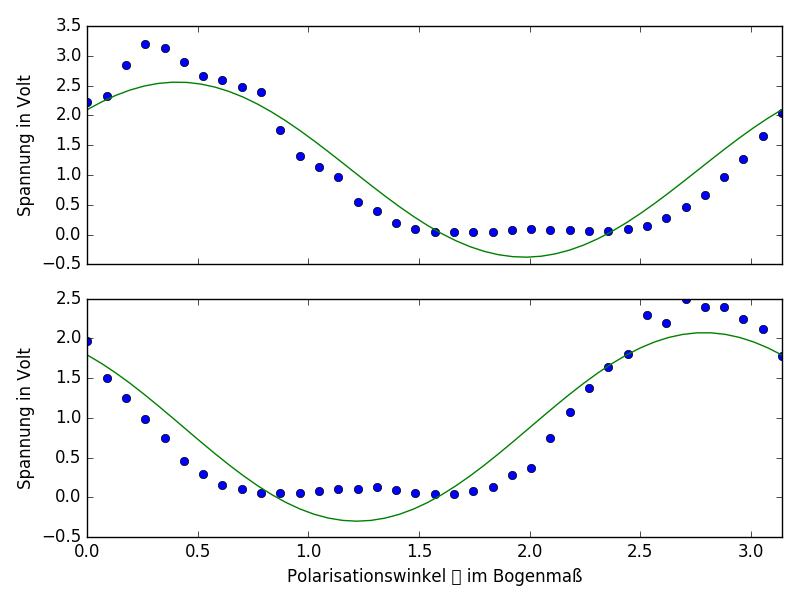
\includegraphics[width=\textwidth]{figures/intensity}
    \caption{Dargestellt sind die Meßwerte und der geschätzte
      funktionale Zusammenhang gemäß \cref{eq:contrast_reg}.  Im oberen
      Plot sind die Meßwerte der maximalen Intensität und im unteren
      Plot diejenigen der minimalen Intensität}
    \label{fig:intensity}
  \end{subfigure}
  \vspace{5mm}

  \begin{subfigure}{0.8\textwidth}
    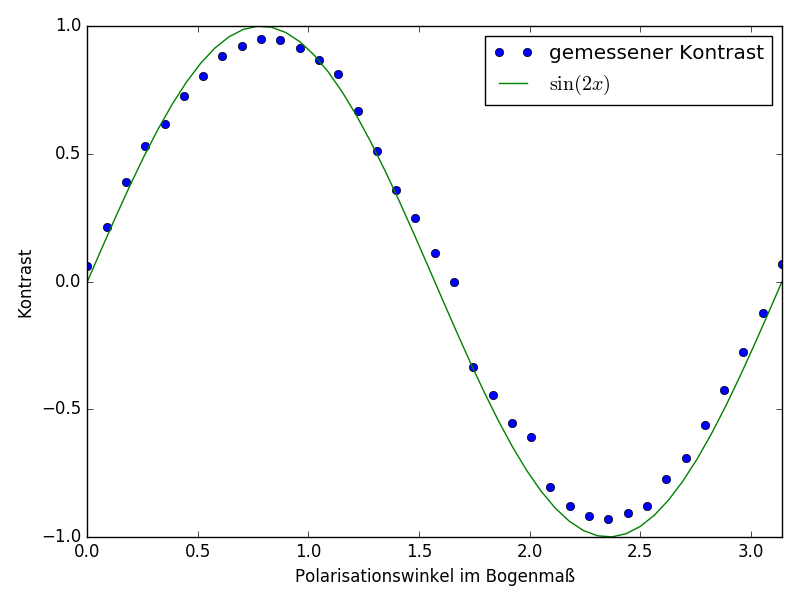
\includegraphics[width=\textwidth]{figures/contrast}
    \caption{Hier ist der Kontrast nach Formel \eqref{eq:kontrast}
      berechnet worden.  Die grüne Kurve zeigt die theoretische
      Erwartung.  Es ist zu erkennen, daß eine gute Übereinstimmung
      vorliegt.}
    \label{fig:contrast}
  \end{subfigure}

  \caption{Graphische Darstellung der Ergebnisse der Kontrastmessung}
\end{figure}

\begin{table}
  \centering
  \begin{tabular}{lSSSSSS}
    \toprule
    & 
    {$A/\si{\volt}$} & {$\frac{\sigma_A}{A}$} &
    {$B$} & {$\frac{\sigma_B}{B}$} &
    {$C/\si{\volt}$} & {$\frac{\sigma_C}{C}$} \\
    \midrule
    Max &
    1.4694 & 0.0566 & 0.7559 & 0.0748 & -0.37826 & 0.2725 \\
    Min &
    1.1867 & 0.0588 & -0.8667 & 0.0681 & -0.3009 & 0.2879\\
    \bottomrule
  \end{tabular}
  \caption{Ergebnisse der Ausgleichsrechnung.  Die Größen $\sigma_i$
    bezeichnen die relativen Standardabweichungen der geschätzten 
    Parameter.  Die Phase $B$ ist im Bogenmaß angegeben.}
  \label{tab:intensity}
\end{table}

\subsection{Messung des Brechungsindex' von Glas}

Die ermittelte Anzahl der $2\pi$-Phasenshifts werden gemäß
\eqref{eq:ref_index_glass} in die entsprechenden Brechindices
umgerechnet.
%
\begin{equation}
  \label{eq:ref_index_glass}
  n = \frac{1}{1 - \frac{\Delta M \lambda_\text{vac}}{T (\Theta_2^2 - \Theta_1^2)}}
\end{equation}
%
Hierbei werden für die Größen $T, \lambda_\text{vac}, \Theta_{1, 2}$ die
Werte aus \cref{tab:tech_data} eingesetzt. Die Formel ergibt sich aus
der Betrachtung der Formel \eqref{eq:glasfringes}.  Die Differenz
\begin{equation}
  \Delta M = M(\Theta_2) - M(\Theta_1) = \frac{2T}{\lambda_\text{vac}}
  \frac{n-1}{2n}\left(\Theta_2^2 - \Theta_1^2\right)
\end{equation}
ist gerade die Anzahl der $2\pi$-Phasenshifts. Durch Umstellen nach $n$
ergibt sich \cref{eq:ref_index_glass}.

Da diese Messung mehrfach durchgeführt worden ist, werden danach das
arithmetische Mittel und die Standardabweichung vom Mittelwert der
enhaltenen Brechindices errechnet.  Es ergibt sich:
%
\begin{equation}
  n = \num{1.4979(0058)}
\end{equation}
%
\begin{table}
  \centering
  \begin{tabular}{SSSSS}
    \toprule
    {$\lambda_\text{vac}/\si{nm}$} & {$T/\si{mm}$} & {$\Theta_1$} &
    {$\Theta_2$} & {$L/\si{mm}$} \\
    \midrule
    632.8 & 1 & 0.1745 & 0.3491 & 100 \\
    \bottomrule
  \end{tabular}
  \caption{Hier sind die Kenngrößen der Apparatur, die in
    \cref{eq:ref_index_glass} eingehen, gelistet.  Die Winkel $\Theta_1,
    \Theta_2$ sind im Bogenmaß angegeben. Hierbei ist $\Theta_1$ der
    Winkel, unter dem die Glasplatten in Strahlrichtung stehen, bevor die
    Platten gedreht werden und $\Theta_2$ der entsprechende Winkel nach
    der Drehung.}
  \label{tab:tech_data}
\end{table}
% 
\subsection{Bestimmung der Brechungsindices von Luft und Kohlendioxid}

Gemäß Formel~\eqref{eq:gasfringes} wird zur gemessenen Anzahl der
$2\pi$-Phasenshifts der Brechungsindex bestimmt.  Die
Apparaturkonstanten sind in \cref{tab:tech_data} angegeben.  In
\cref{tab:gas} sind die Ergebnisse eingetragen und in \cref{fig:gas}
graphisch dargestellt.

Da der Plot der Meßdaten die Vermutung nahe legt, daß die Meßpunkte auf
einer Geraden liegen, nehmen wir eine lineare
Regressionsrechnung\footnote{%
  Zur Bestimmung der Parameter verwenden wir die Funktion
  \texttt{scipy.stats.linregress} aus der \texttt{scipy}-Bibliothek in
  der Version 0.10.1}
%
vor.  Die Ergebnisse für die Parameter sind in \cref{tab:linreg}
dargestellt, außerdem sind entsprechende Ausgleichsgeraden in
\cref{fig:gas} eingezeichnet.  Mit Hilfe der Ausgleichsgeraden werden
Werte für die Brechungsindices von Luft und Kohlendioxid bei Normaldruck
bestimmt. Die Ergebnisse sind ebenfalls in \cref{tab:linreg} zu finden.
Zur Fehlerabschätzung sind in der Gleichung $n = \beta_0 p + \beta_1$
die Steigung $\beta_0$ und der Achsenabschnitt $\beta_1$ als
fehlerbehaftet betrachet.  Eine \name{Gauß}sche Fehlerfortpflanzung
liefert für den Fehler des Brechungsindex
%
\begin{equation}
  \sigma_n = \sqrt{p^2 \sigma_{\beta_0}^2 + \sigma_{\beta_1}^2}
\label{eq:ref_index_error}
\end{equation}


\begin{table}
  \centering
  \sisetup{
    table-figures-integer  = 2,
    table-figures-decimal  = 5,
    table-figures-uncertainty = 5,
    table-number-alignment = center,
    retain-unity-mantissa  = false
  }
  \begin{tabular}{SSSS}
    \toprule
    {$\beta_0/\SI{1e-7}{\per\milli\bar}$} &
    {$\sigma_{\beta_0}/\SI{1e-7}{\per\milli\bar}$} &
    {$\beta_1$} &
    {$\sigma_{\beta_0}/10^{-13}$} \\
    \midrule
    2.71432 & 0.00578 & 0.99999 & 6.22043 \\

    2.63442 & 0.00539 & 0.99999 & 5.80418 \\

    3.47466 & 0.00972 & 0.99999 & 10.4682 \\
    \midrule
    & & \multicolumn{2}{c}{Brechungsindex}\\
    \midrule
    \multicolumn{2}{l}{Luft bei \SI{1000}{\milli\bar} (1. Messung)} &
    \multicolumn{2}{S[table-figures-decimal  = 8,
    table-figures-uncertainty = 8]}{1.00025898(58)} \\
    \multicolumn{2}{l}{Luft bei \SI{1000}{\milli\bar} (2. Messung)} &
    \multicolumn{2}{S[table-figures-decimal  = 8,
    table-figures-uncertainty = 8]}{1.00025235(54)} \\
    \multicolumn{2}{l}{Kohlendioxid bei \SI{1000}{\milli\bar}}      &
    \multicolumn{2}{S[table-figures-decimal  = 8,
    table-figures-uncertainty = 8]}{1.00033211(97)} \\
    \bottomrule
  \end{tabular}

  \caption{Der Ergebnisse der linearen Ausgleichsrechnung.  Die Parameter
    bezeichnen die Steigung $\beta_0$ und den y-Achsenabschnitt $\beta_1$
    der Ausgleichsgeraden.  Der Fehler des Brechungsindex wird nach
    \cref{eq:ref_index_error} berechnet.}
  \label{tab:linreg}
\end{table}

\begin{figure}
  \centering
  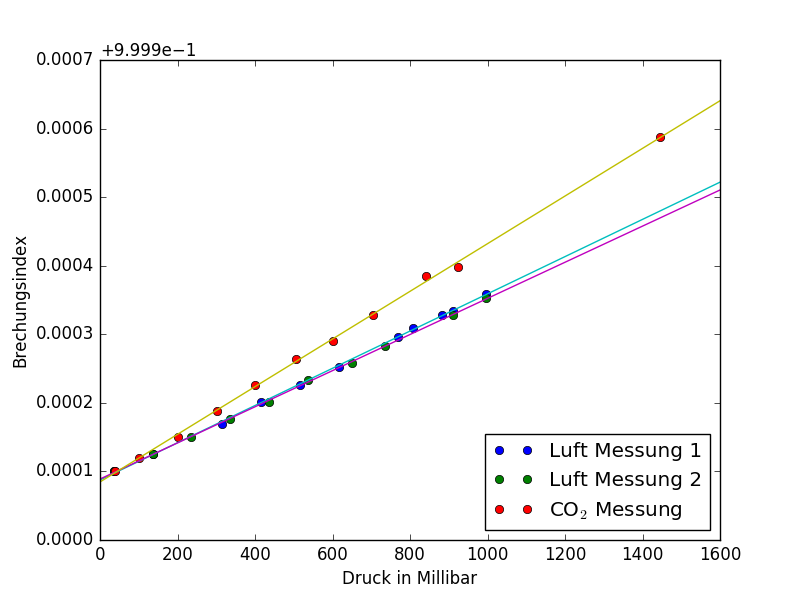
\includegraphics[width=0.8\textwidth]{figures/pressure-ref-index.pdf}
  \caption{Graphische Darstellung der errechneten Brechungsindices von
    Luft und Kohlendioxid.  Die Meßpunkte liegen näherungsweise auf den
    eingezeichneten Regressionsgeraden.}
  \label{fig:gas}
\end{figure}

\begin{table}
  \centering\footnotesize
  \sisetup {
    scientific-notation = fixed,
    fixed-exponent      = 0
  }
  \begin{subtable}{0.3\textwidth}
    \begin{tabular}{SS}
      \toprule
      {$p/\si{\milli\bar}$} & {Brechungsindex}\\
      \midrule
       36 & 1.00000 \\
      136 & 1.00003 \\
      316 & 1.00007 \\
      416 & 1.00010 \\
      516 & 1.00013 \\
      616 & 1.00015 \\
      770 & 1.00020 \\
      807 & 1.00021 \\
      882 & 1.00023 \\
      912 & 1.00023 \\
      996 & 1.00026 \\
      \bottomrule
    \end{tabular}
    \caption{Luft, 1. Meßreihe}
  \end{subtable}
  \quad
  \begin{subtable}{0.3\textwidth}
    \begin{tabular}{SS}
      \toprule
      {$p/\si{\milli\bar}$} & {Brechungsindex}\\
      \midrule
       36 & 1.00000 \\
      136 & 1.00003 \\
      236 & 1.00005 \\
      336 & 1.00008 \\
      436 & 1.00010 \\
      536 & 1.00013 \\
      650 & 1.00016 \\
      736 & 1.00018 \\
      911 & 1.00023 \\
      996 & 1.00025 \\
      \\
      \bottomrule
    \end{tabular}
    \caption{Luft, 2. Meßreihe}
  \end{subtable}
  \quad
  \begin{subtable}{0.3\textwidth}
    \begin{tabular}{SS}
      \toprule
      {$p/\si{\milli\bar}$} & {Brechungsindex}\\
      \midrule
        38 & 1.00000 \\
       101 & 1.00002 \\
       201 & 1.00005 \\
       301 & 1.00009 \\
       401 & 1.00013 \\
       506 & 1.00016 \\
       600 & 1.00019 \\
       704 & 1.00023 \\
       840 & 1.00028 \\
       923 & 1.00030 \\
      144  & 1.00049 \\
      \bottomrule
    \end{tabular}
    \caption{Kohlendioxid}
  \end{subtable}
  
  \caption{Die Brechungsindices von Luft und Kohlendioxid in
    Abhängigkeit vom Druck.}
  \label{tab:gas}
\end{table}  
